\chapter*{Introducción}
\epigraph{Per aspera ad astra.}{\textit{Lucio Anneo Séneca}}
%\epigraph{A caballo regalado no se le mira el diente.}{\textit{}}
Los números $p$-ádicos fueron recientemente introducidos por \textit{K. Hensel} en las matemáticas modernas con el fin de solucionar varios problemas en la teoría de números. Como consecuencia, el desarrollo del análisis $p$-ádico se ha visto involucrado en otras ramas de la ciencia, como la Biología, en donde los fenómenos naturales son presentados como estructuras jerárquicas \cite{Av-5}; en la Física, donde juegan un papel importante en la teoría de cuerdas \cite{Dragovich-2017}; y por supuesto, en las Ciencias de la computación, en donde son usados para hacer \textit{Data Mining} y \textit{Criptografía} \cite{Dragovich-2017}.

En este trabajo explicaremos algunas nociones básicas de análisis en espacios ultramétricos, en particular en el cuerpo de números $p$-ádicos. De esta manera mostraremos una representación visual de los mismos, con el fin de desarrollar un paquete amigable que pueda ser implementado por científicos para hacer cómputo $p$-ádico (por ejemplo en la codificación de información) y desarrollar simulaciones de ecuaciones presentes en sistemas complejos.

En el Capítulo \ref{chapter1} fijamos la notación y presentamos algunos resultados básicos sobre el análisis  $p$-ádico, que serán utilizados a lo largo de este trabajo. Para una exposición más completa  sobre el análisis $p$-ádico  el
lector puede consultar  \cite{A-K-S}, \cite{Taibleson}, \cite{Koch}, \cite{V-V-Z}.

Dado que el interés principal de este trabajo está enfocado al uso computacional de los números $p$-ádicos y dado que existen paquetes ofrecidos por \texttt{Mathematica} para hacer cómputos aritméticos de números $p$-ádicos, encontramos que estos cómputos en general son puntuales, es decir, son operaciones número a número; luego, la representación gráfica de los mismos queda en segundo plano. Además, la última fecha de revisión de los algoritmos es del año 1996\footnote{\url{https://library.wolfram.com/infocenter/MathSource/556/}}; razón por la cual requerimos de una forma amigable y eficente\footnote{La eficiencia basada en el concepto de complejidad algorítmica.} de realizar estos cómputos.

En el Capítulo \ref{chapter2} se propone un diseño orientado a objetos (ya que es el paradigma de programación más común) para números $p$-ádicos; además, consideramos una implementación en \texttt{Python}\footnote{Se requiere el uso de Python 3.5 en adelante. Ver \ref{apendice} para más requerimientos.}, dado que presenta características deseables como ser moderno, orientado a objetos, ser de uso común por la mayoría de científicos, así como poseer frameworks y poseer estructuras de datos que permiten, a diferencia de otros lenguajes, una manipulación más simple de grafos y redes. Más específicamente, nos basamos en un paquete abierto, ofrecido por la comunidad de desarrolladores, llamado \texttt{NetworkX}\footnote{Para una documentación detallada acerca del paquete visitar: \url{https://networkx.github.io/documentation/latest/_downloads/networkx_reference.pdf}}, dedicado a la creación, manipulación, estudio de estructuras, funciones y dinámica de redes complejas.

La natulareza nos presenta varios tipos de estructuras jerárquicas; por ejemplo en los sistemas complejos, los cristales, clústeres y proteínas son objetos de estudio. Ver por ejemplo \cite{Av-3,A-B-O,Av-5}. Luego, se hace conveniente tratar de tener una noción acerca de los sistemas complejos. Un sistema complejo es un grupo formado por componentes que interactúan entre sí, con algunas configuraciones que, en el caso de proteínas, tienen asociadas funciones de energía.

Esta noción introductoria nos lleva finalmente al Capítulo \ref{chapter_3} con el fin de estudiar la jerarquía ultramétrica presente en el estudio de proteínas (ver por ejemplo \cite{Av-5}), por medio de aproximaciones de estructuras asociadas a las mismas y afines a la representación dada en el Capítulo \ref{chapter2}.

Por último, desarrollamos el Apéndice \ref{apendice} donde explicamos al lector cómo instalar el paquete a través del uso del \textit{sistema de gestión de paquetes} escritos en \texttt{Python} (\texttt{pip}); añadiento que es la primera versión de código abierto para seguir desarrollando algoritmos no incluidos en este trabajo, por ejemplo, los relacionados al estudio algebraico de los números $p$-ádicos. 
\newpage
\section*{Breve reseña de Hensel}
%\begin{multicols}{2} \columnbreak
\begin{center}
	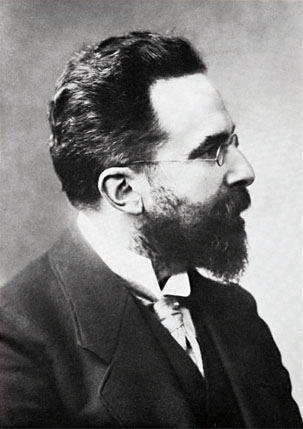
\includegraphics[scale = 0.76]{img/kurt_hensel.jpg}
\end{center}
	
	\textbf{Kurt Hensel} Nació el 29 de diciembre de 1861 en lo que se conoció como Könisberg, Prusia. A finales del siglo XIX y teniendo influencias de profesores como \textit{ Lipschitz, Weierstrass, Borchardt, Kirchhoff, Helmholtz y Kronecker}; este último motivó el estudio del método de Weierstrass en series de potencias de funciones consiguiendo introducir los números $p$-ádicos, $\Qp$. Su interés inicial estaba en encontrar la potencia exacta de un primo que dividiera el \textit{discriminante} de un cuerpo de números\footnote{El discriminante de un cuerpo de números es un invariante numérico que "mide" el tamaño de el anillo de enteros del cuerpo.}.\\
	
	Más adelante, introdujo el concepto de cuerpo con valuación, que luego tendría gran influencia en el estudio del álgebra moderna. Desde esta época, la popularidad de los números $p$-ádicos creció sin parar, y durante el siglo XX hasta hoy en día se sigue desarrollando la inmensa teoría que de fondo llevan a ramas de estudio como la teoría de números y aplicaciones \cite{Av-1}. 
	
%\end{multicols}{2}
